\subsubsection{Adapted SAGAT}
\label{subsubsec:results_adapted_sagat_1}

This section discusses the results of the adapted SAGAT questionnaire, which aims at assessing the participant's situation awareness and their mental map of the environment. 

For each question of the SAGAT questionnaire, the participant could score 1 point or a fraction of it. The total score achieved by each blind participant is presented in Table \ref{tab:sagat_table_blind}. Figure  \ref{fig:barplot_sagat_avg_5_scene_blind} illustrates the corresponding bar plot, indicating the mean and standard deviation for each guidance method and each round. This figure shows clearly that the participants improved their situation awareness in the return round, when they already had some information about the environment. Also, it is possible to observe that the worst situation awareness is obtained in the first round for the virtual cane. However, on the return round, the SAGAT mean score becomes equivalent to the audio method.


\begin{table}[!htb]
\centering
\caption{SAGAT global score felled by the blinded participants.}
\label{tab:sagat_table_blind}
\begin{tabular}{llrrrrr}
\toprule
     &        &   Base &  Audio & \begin{tabular}[c]{@{}l@{}}Haptic\\ Belt\end{tabular} & \begin{tabular}[c]{@{}l@{}}Virtual\\ Cane\end{tabular} & Mixture \\
Participant & Round &        &        &                                                       &                                                        &         \\
\midrule
001C & First &   6.25 &   5.50 &                                                  5.33 &                                                   5.83 &   3.500 \\
     & Return &   6.25 &   6.50 &                                                  8.50 &                                                   5.50 &   5.500 \\
002C & First &   6.75 &   4.50 &                                                  3.99 &                                                   4.50 &   6.250 \\
     & Return &   5.25 &   5.00 &                                                  4.00 &                                                   6.50 &   8.500 \\
003C & First &   7.25 &   7.50 &                                                  7.49 &                                                   4.66 &   9.000 \\
     & Return &  10.00 &  10.00 &                                                  8.50 &                                                   9.00 &   9.000 \\
004C & First &   7.50 &   6.00 &                                                  7.66 &                                                   4.99 &   6.500 \\
     & Return &   9.00 &   6.00 &                                                  9.25 &                                                   7.25 &   9.000 \\
\bottomrule
\end{tabular}
\end{table}



\begin{figure}[!htb]
    \centering
    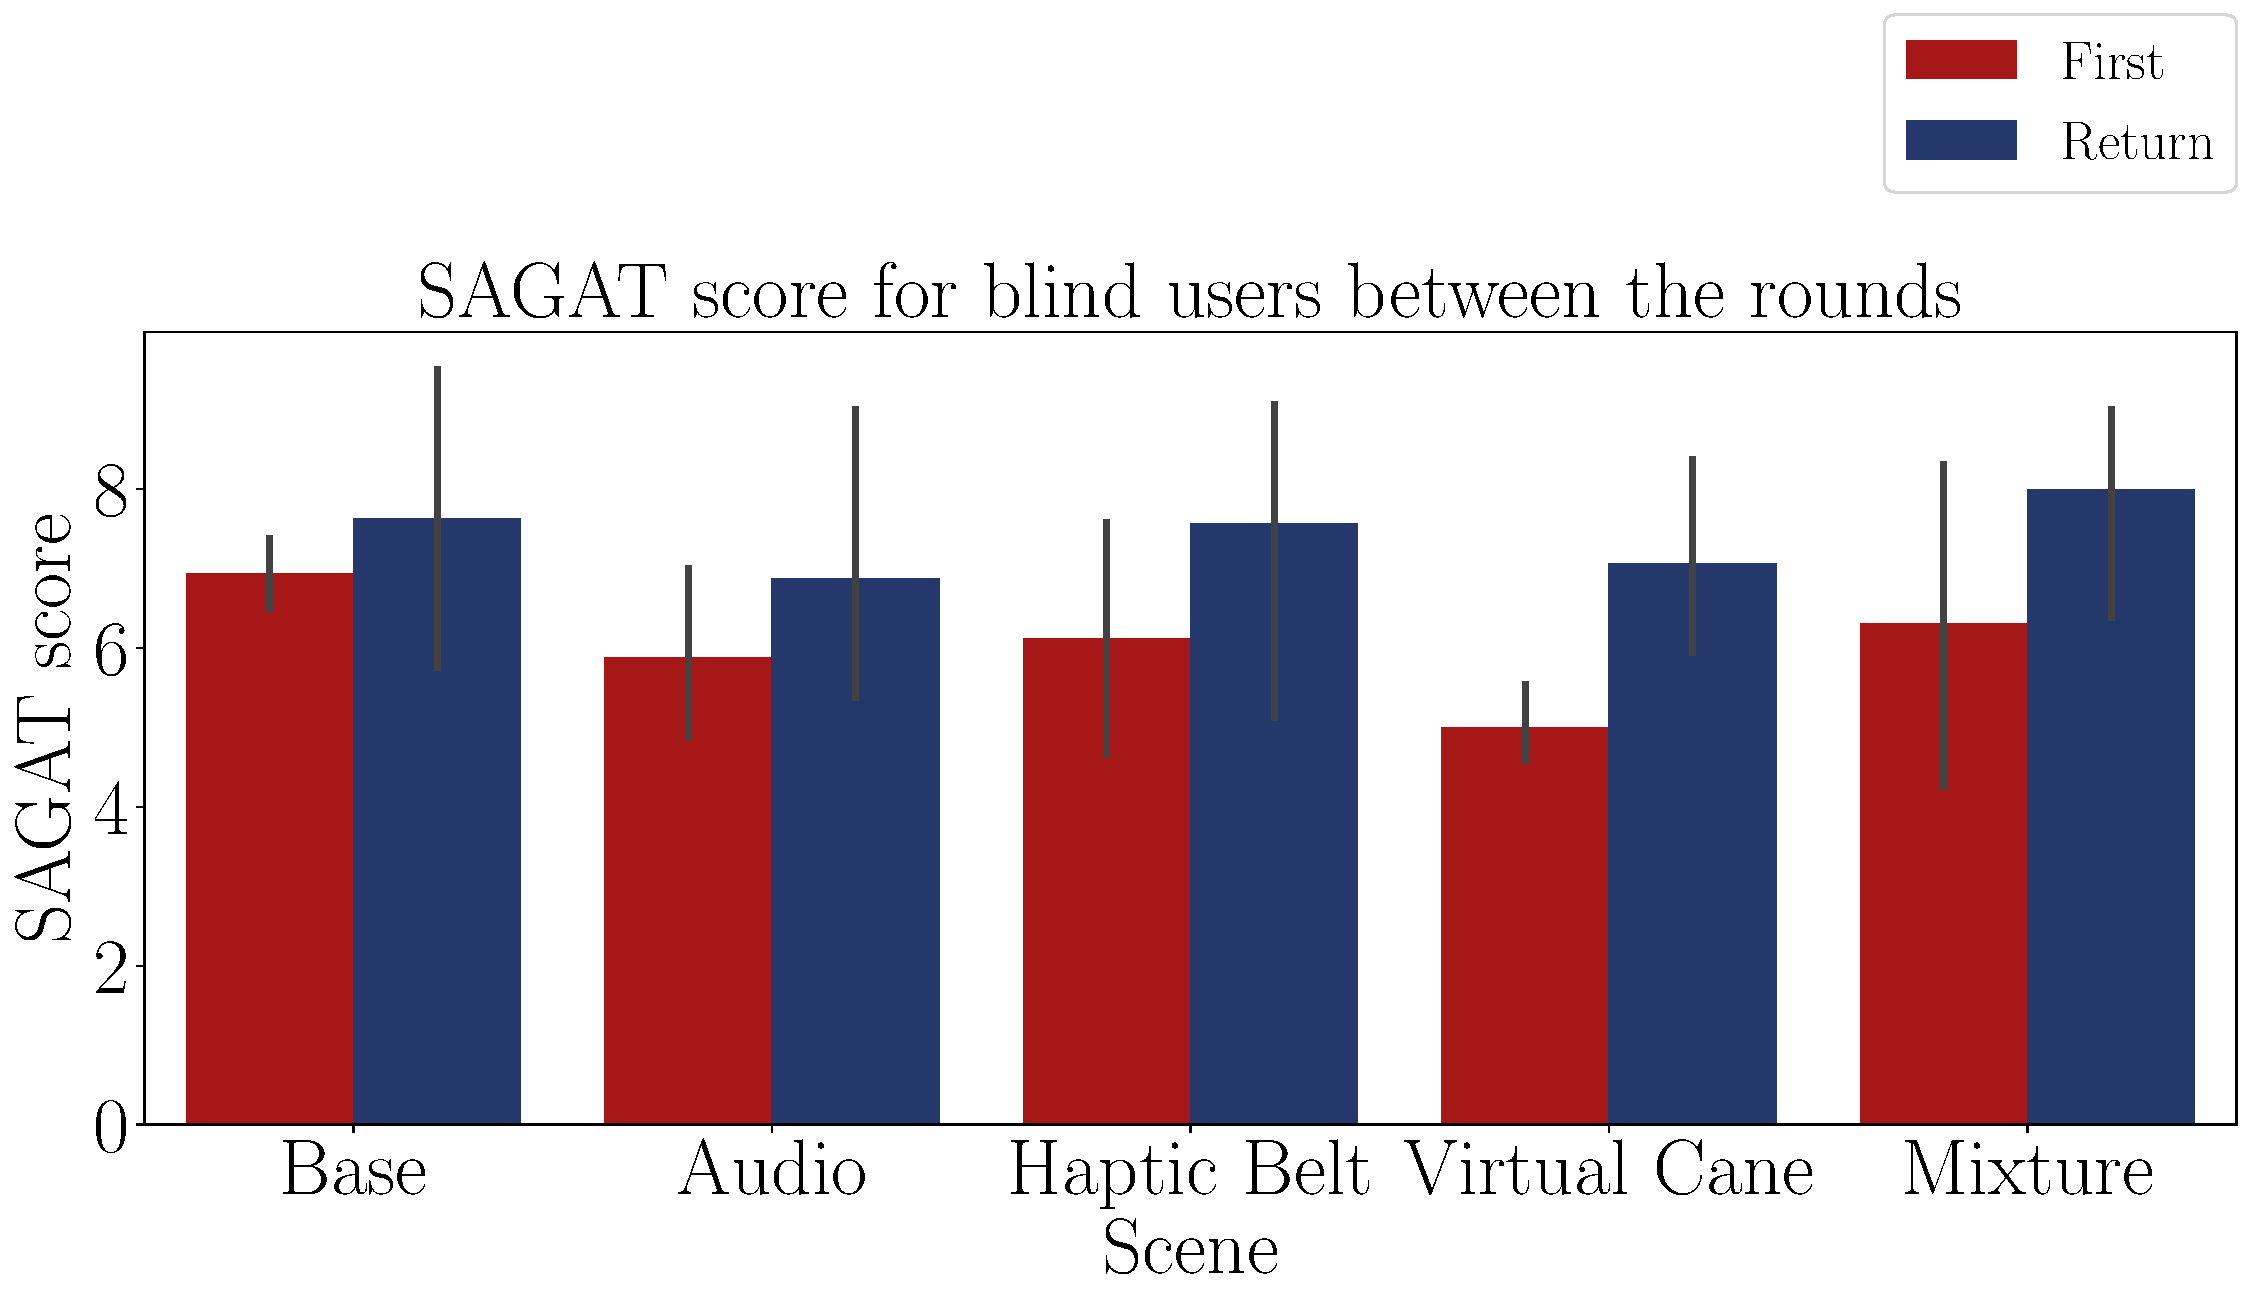
\includegraphics[width = \textwidth]{Resultados/Sagat/Figuras/pdf/barplot_sagat_avg_5_scene_blind.pdf}
    \caption{Barplot of the average SAGAT score of the blind participants on each method.}
    \label{fig:barplot_sagat_avg_5_scene_blind}
\end{figure}

Figure \ref{fig:boxplot_sagat_blind_scene} brings the boxplot of the SAGAT score grouped by the guidance methods. It shows that the methods can be divided into two groups. The first one is composed of base, haptic belt and the mixture. This group received scores higher than the second group, composed of audio and virtual cane. Figure \ref{fig:boxplot_sagat_blind_rounds} shows the boxplot of the data grouped by round and confirms the general improvement of situation awareness from the first to the return round. 

\begin{figure}[!htb]
    \centering
    \begin{minipage}{0.45\textwidth}
        \centering
        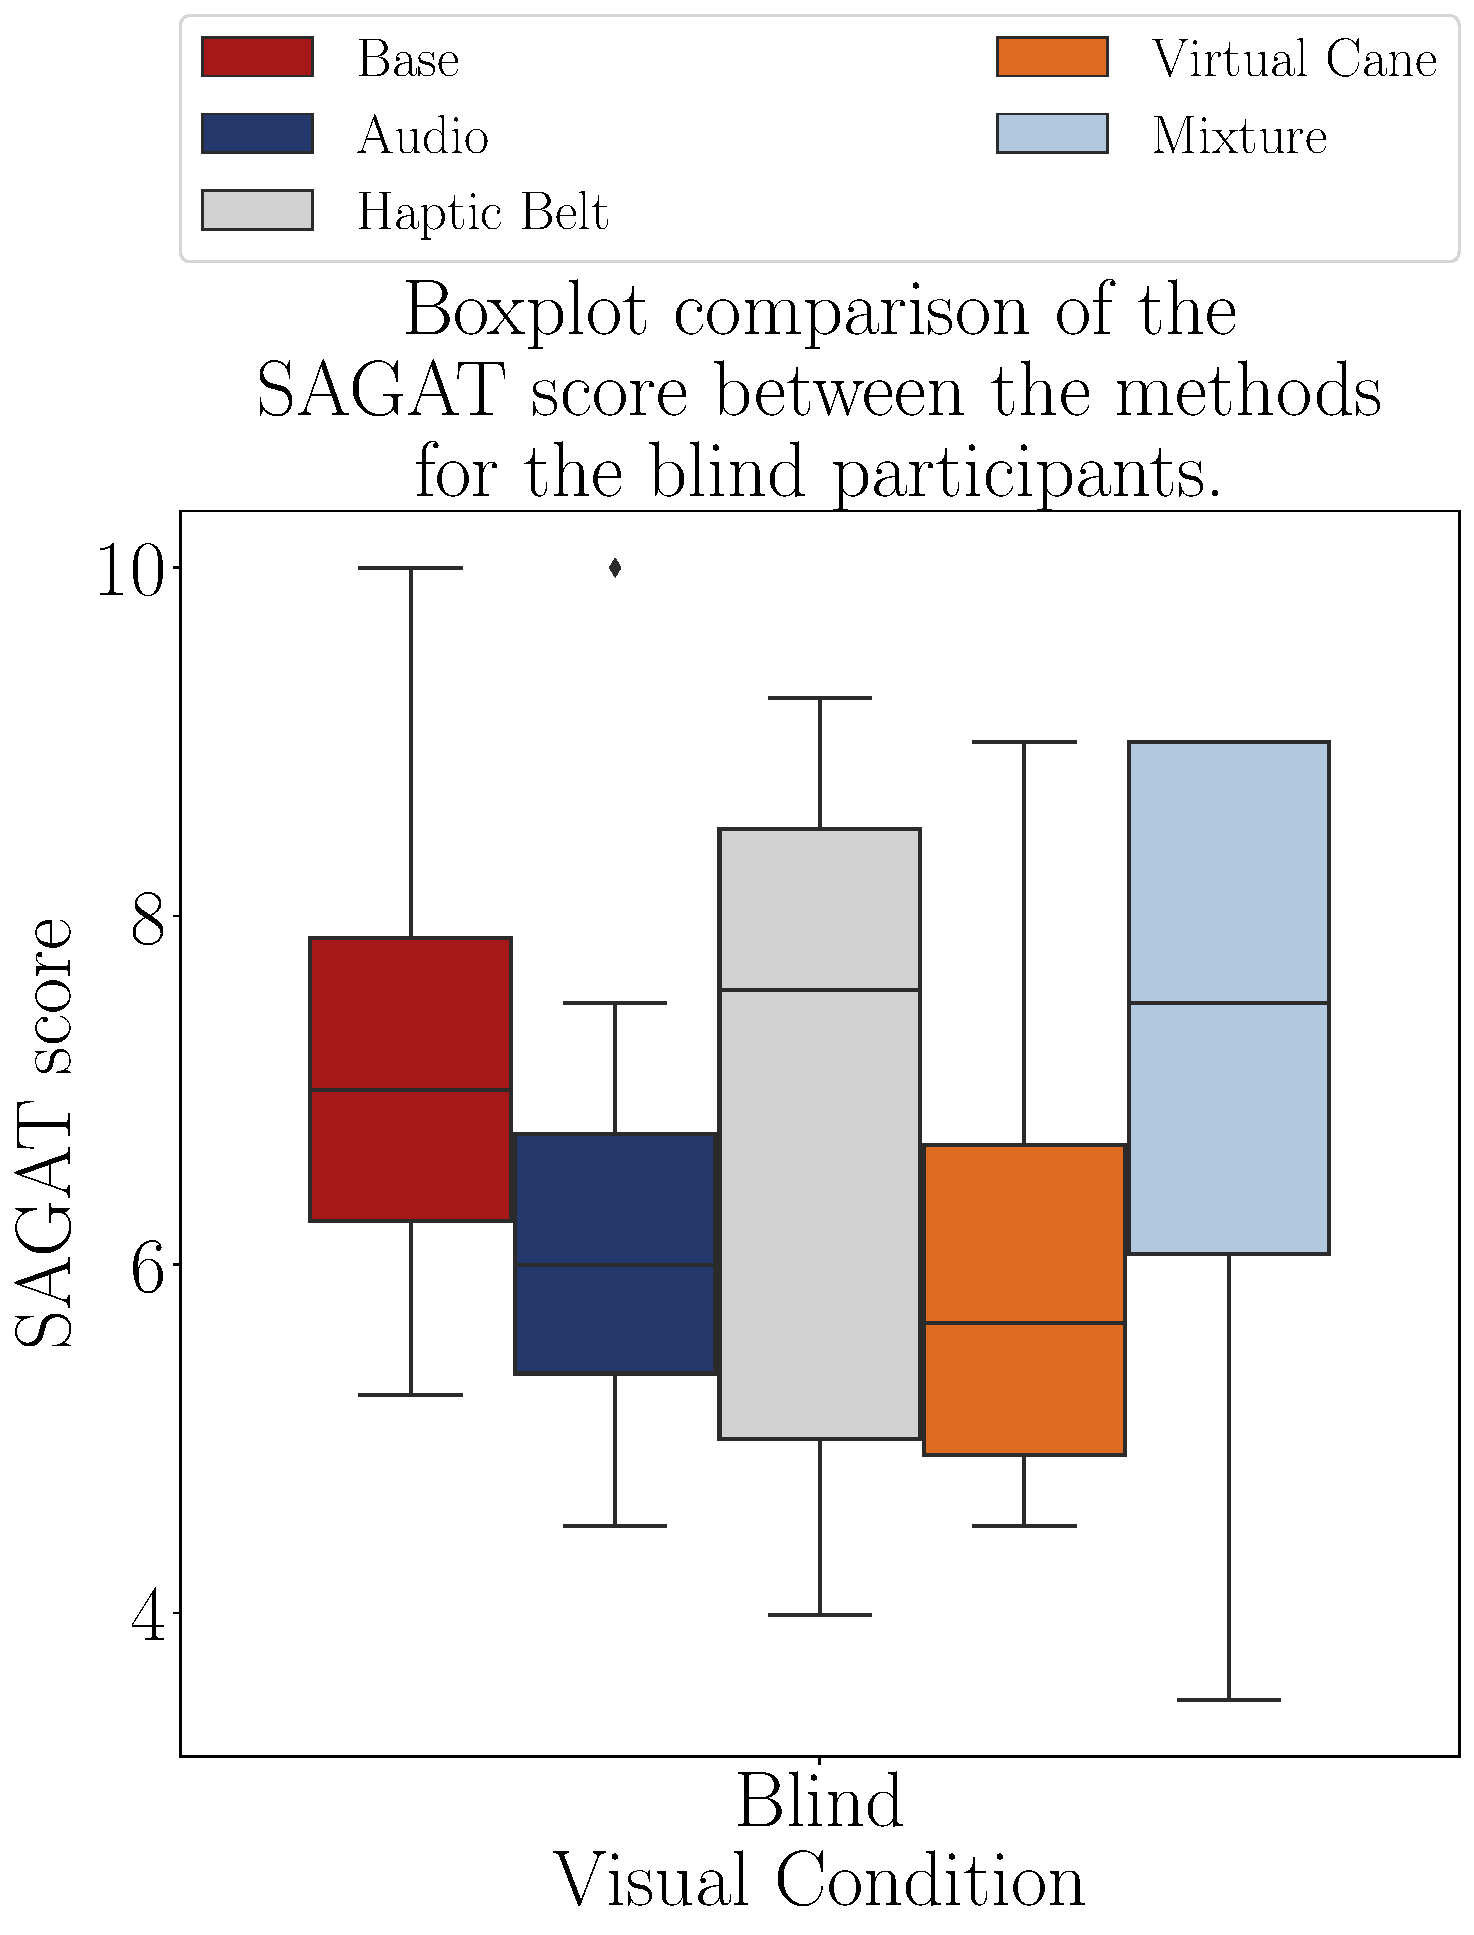
\includegraphics[width = \textwidth]{Resultados/Sagat/Figuras/pdf/boxplot_sagat_blind_scene.pdf}
        \caption{Boxplot of the SAGAT score of the blind participants grouped by the methods.}
        \label{fig:boxplot_sagat_blind_scene}
    \end{minipage}
    \begin{minipage}{0.075\textwidth}
        \hfill
    \end{minipage}
    \begin{minipage}{0.45\textwidth}
        \centering
        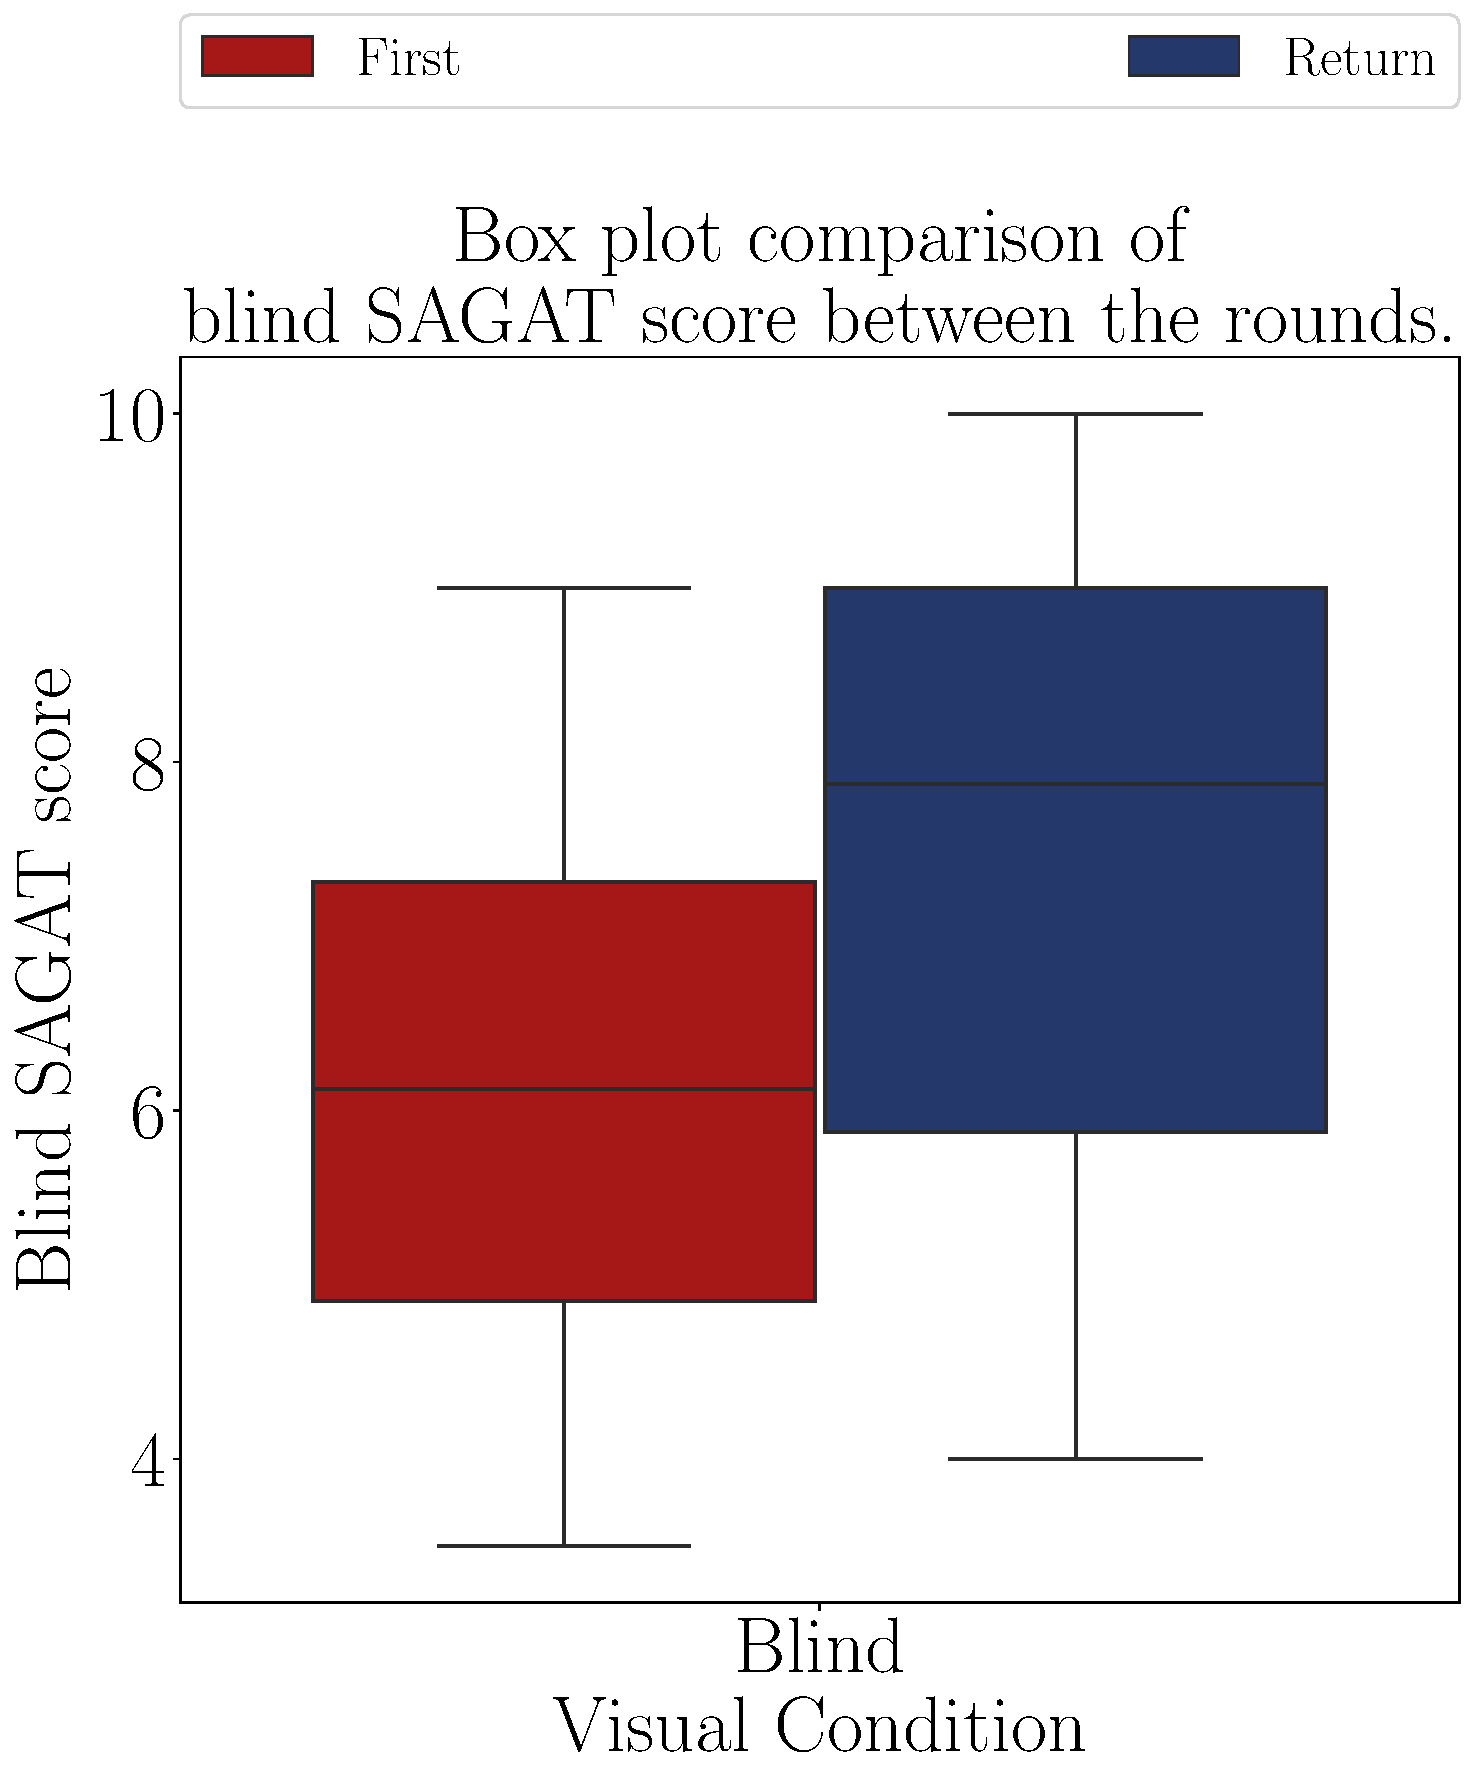
\includegraphics[width = \textwidth]{Resultados/Sagat/Figuras/pdf/boxplot_sagat_blind_rounds.pdf}
        \caption{Boxplot of the SAGAT score of the blind participants grouped by the rounds.}
        \label{fig:boxplot_sagat_blind_rounds}
    \end{minipage}
\end{figure}

Proceeding to the statistical analysis of the data, Figures \ref{fig:qqplot_sagat_avg_two_way_blind} and \ref{fig:residplot_sagat_avg_two_way_blind} present the QQ plot and the residual distribution, which confirms the normal distribution assumption and the homogeneity of variances.

\begin{figure}[!htb]
    \centering
    \begin{minipage}{0.45\textwidth}
        \centering
        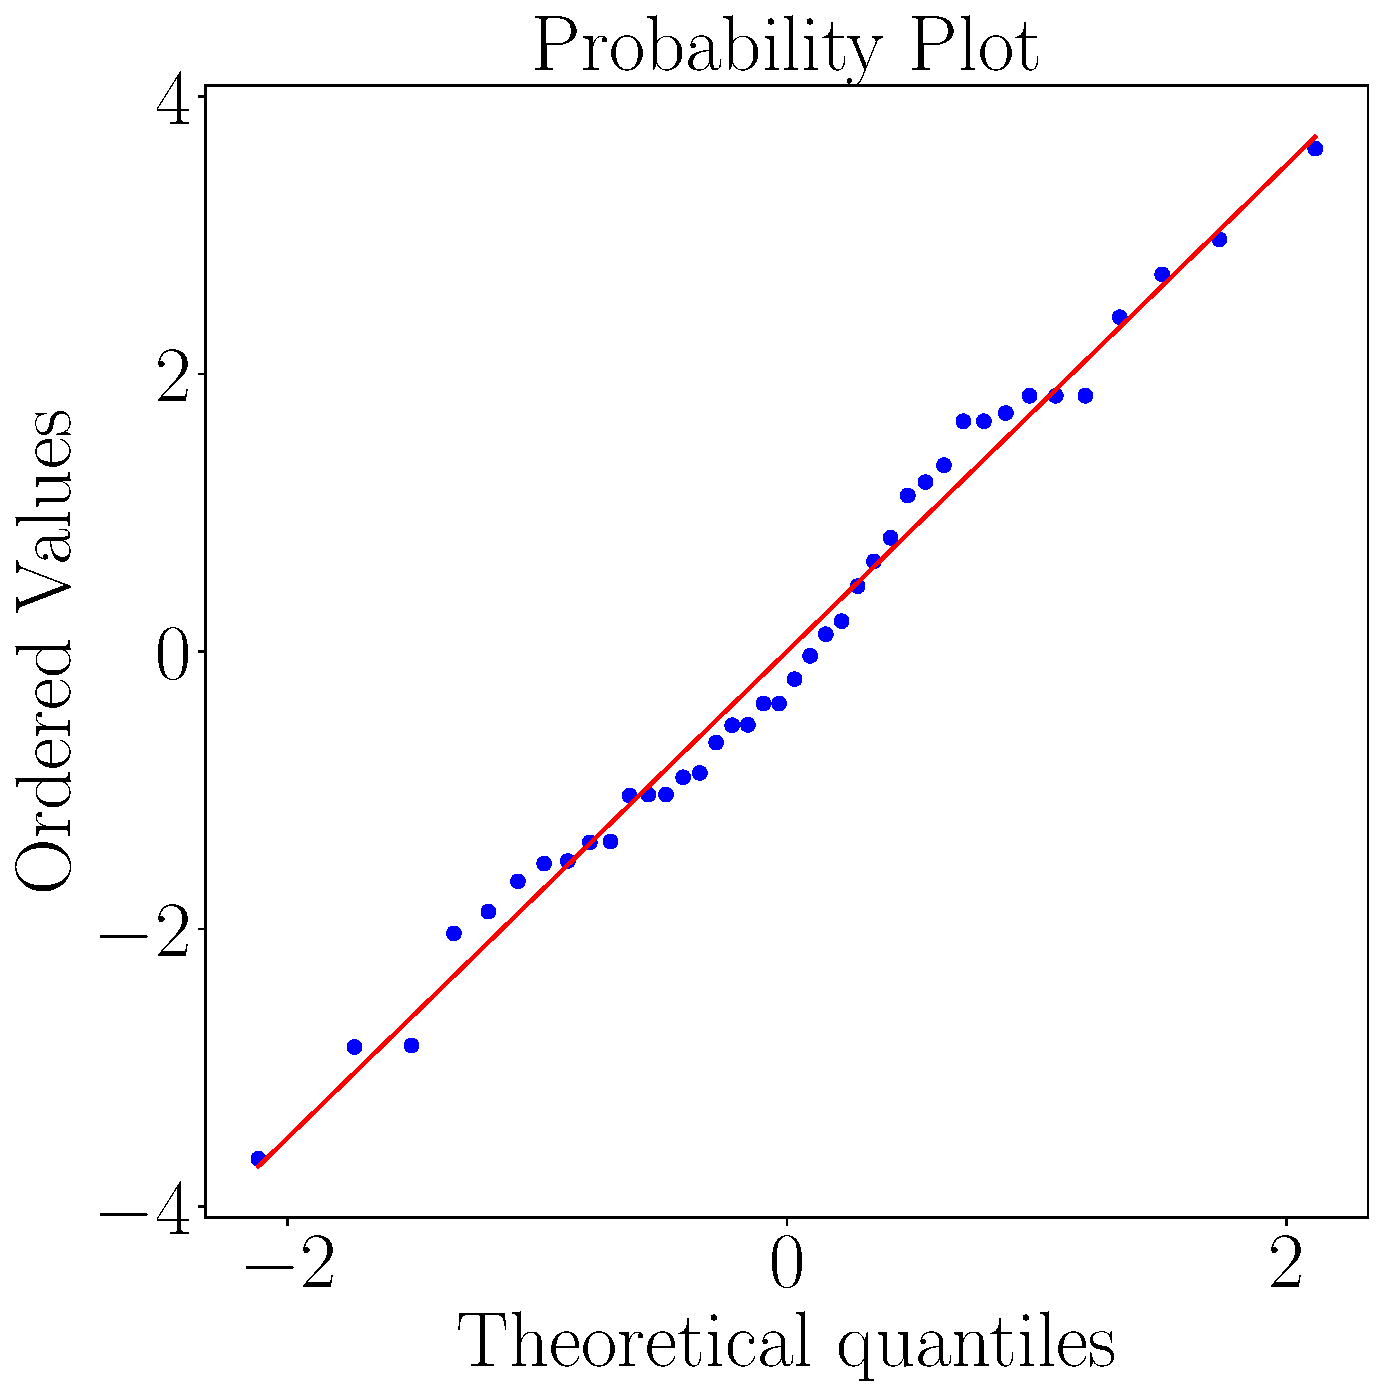
\includegraphics[width = \textwidth]{Resultados/Sagat/Figuras/pdf/qqplot_sagat_avg_two_way_blind.pdf}
        \caption{QQ plot of the SAGAT score of the blind participants on each method.}
        \label{fig:qqplot_sagat_avg_two_way_blind}
    \end{minipage}
    \begin{minipage}{0.075\textwidth}
        \hfill
    \end{minipage}
    \begin{minipage}{0.45\textwidth}
        \centering
        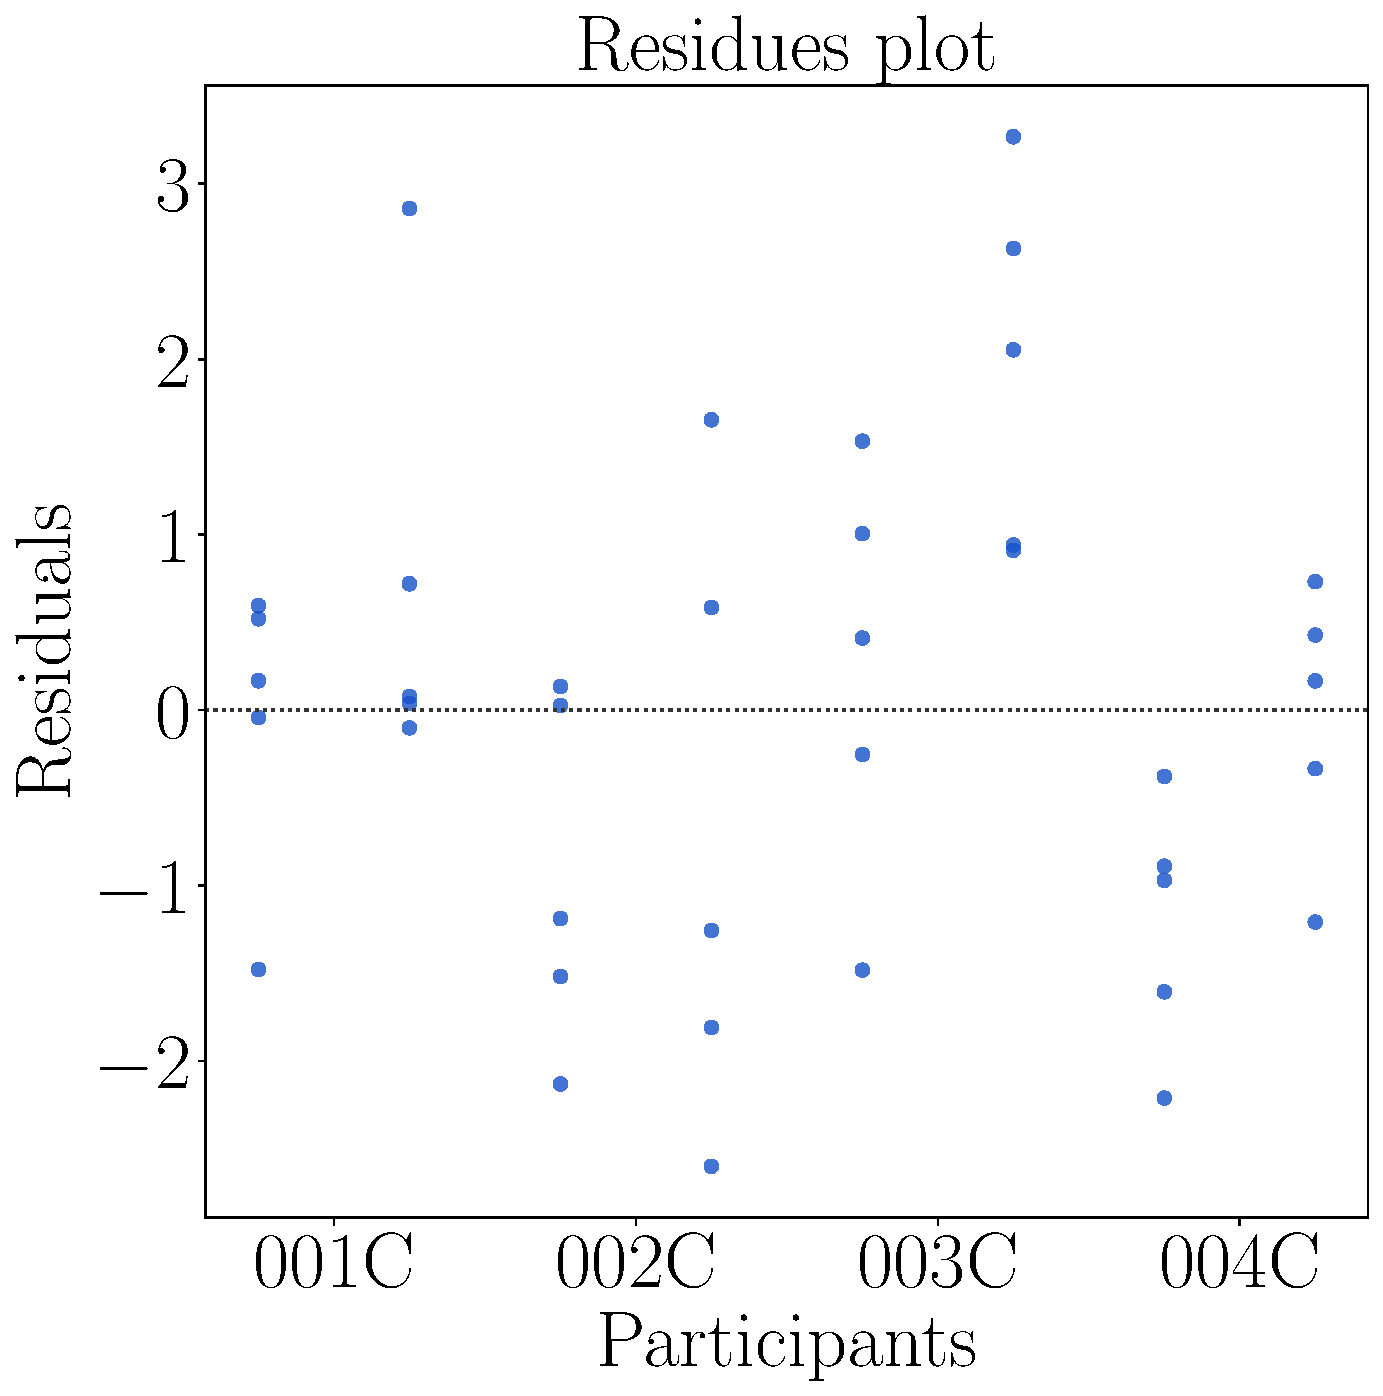
\includegraphics[width = \textwidth]{Resultados/Sagat/Figuras/pdf/residplot_sagat_avg_two_way_blind.pdf}
        \caption{Residual plot of the SAGAT score the blind participants on each method.}
        \label{fig:residplot_sagat_avg_two_way_blind}
    \end{minipage}
\end{figure}

Table \ref{tab:blocanova_sagat_avg_two_way_blind} shows the ANOVA test p-value of the SAGAT score. It indicates that the round is a significant variable that influences the value of the SAGAT score. The same cannot be said for the method, which has no significant influence.


\begin{table}[!htb]
\centering
\caption{Anova p-value for the SAGAT score on each method for blinded users.}
\label{tab:blocanova_sagat_avg_two_way_blind}
\begin{tabular}{lrrrrr}
\toprule
               Source &  Squared sum &  DOF & Squared average &      F & \begin{tabular}[c]{@{}l@{}}P-Value \\ $(F_{0} > F)$\end{tabular} \\
\midrule
Participants (Blocks) &       48.231 &    3 &          16.077 &  9.731 &                                                                  \\
         \    Methods &        8.922 &    4 &           2.230 &  1.350 &                                                            0.277 \\
          \    Rounds &       18.975 &    1 &          18.975 & 11.485 &                                                          0.002** \\
     \    Interaction &        2.391 &    4 &           0.598 &  0.362 &                                                            0.834 \\
   Experimental Error &       44.608 &   27 &           1.652 &        &                                                                  \\
                Total &      123.127 &   39 &                 &        &                                                                  \\
\bottomrule
\end{tabular}
\end{table}



Finally, Table \ref{tab:sagat_var_group_blind} presents the mean difference in the SAGAT score between the first and return rounds for each guidance method. It shows that the base and audio methods have the lowest difference, while the highest was obtained for the virtual cane.


\begin{table}[!htb]
\centering
\caption{Adapted Sagat global score variation grouped by participant and visual Condition}
\label{tab:sagat_var_group_blind}
\begin{tabular}{lrrrrrr}
\toprule
{} &  Base &  Audio & \begin{tabular}[c]{@{}l@{}}Haptic\\ Belt\end{tabular} & \begin{tabular}[c]{@{}l@{}}Virtual\\ Cane\end{tabular} & Mixture \\
Visual Condition &       &        &                                                       &                                                        &         \\
\midrule
Blind            &  8.93 &  15.66 &                                                 23.49 &                                                  44.30 &   32.90 \\
\bottomrule
\end{tabular}
\end{table}



\FloatBarrier